\section{The TEPX upgrade for HL-LHC}
\label{sec:tepx}
(describe the TEPX detector design, algorithms clusters/coincidences, stat precision, linearity)\\

The High Luminosity (HL)-LHC will increase instantaneous luminosity to unprecedented values of $7 \times 10^{34} cm^{-2} s^{-1}$ which corresponds to 200 proton-proton collisions per bunch crossing (pileup). Run 2 pixel detector will not be able to handle the extreme radiation environment, resolve nearby particle tracks and operate properly for high pileup values. That is why Run 2 pixel detector will be replaced by a new pixel detector which will be composed of three subdetectors: tracker barrel pixel detector (TBPX), tracker forward pixel detector (TFPX) and tracker endcap pixel detector (TEPX).

\begin{figure}[H]
  \centering
  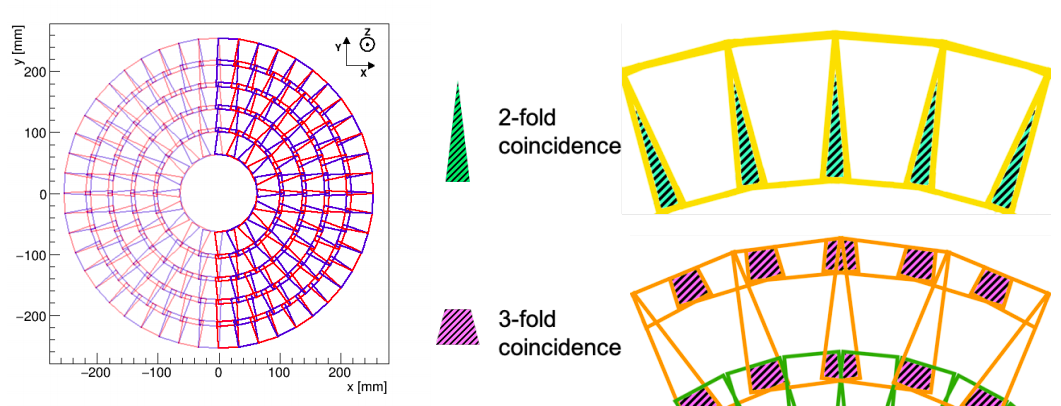
\includegraphics[width=0.6\columnwidth]{./up.png}
  \caption{\onehalfspacing Left: View in the x-y plane of the double disk structure of one TEPX disk. The sensors in blue and red correspond to the two double disks at slightly different z positions. Right: Example of two- and threefold coincidence regions on a portion of a single TEPX disk \cite{}.}
  \label{fig:CMS}
\end{figure}


\begin{figure}[H]
  \centering
  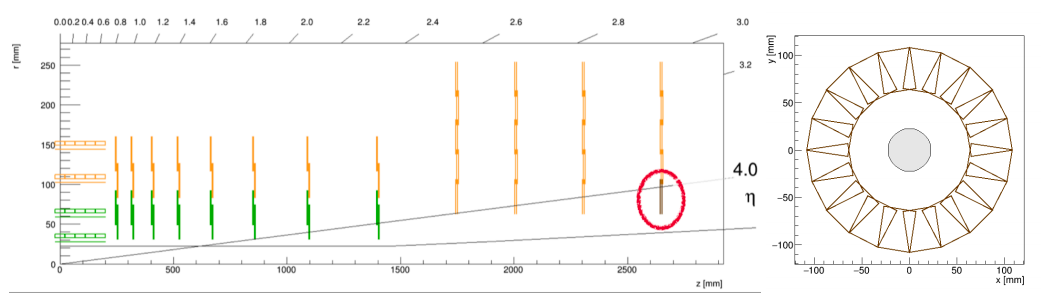
\includegraphics[width=0.6\columnwidth]{./up1.png}
  \caption{ \onehalfspacing Left: A layout of the CMS Phase-2 inner tracker with the location of TEPX Disk 4, Ring 1 highlighted in dark red. Right: The x-y view of TEPX disk 4, ring 1 \cite{}.}
  \label{fig:CMS}
\end{figure}


\begin{figure}[H]
  \centering
  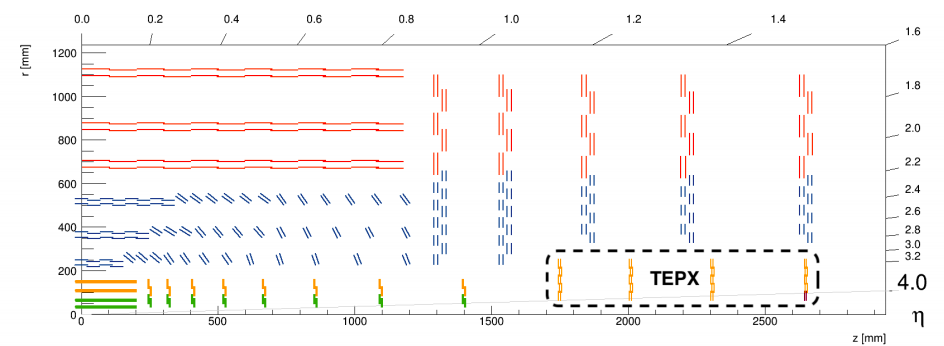
\includegraphics[width=0.6\columnwidth]{./up2.png}
  \caption{ \onehalfspacing Schematic view for one quarter of the tracker, illustrating the location of TEPX. \cite{}.}
  \label{fig:CMS}
\end{figure}


\begin{figure}[H]
  \centering
  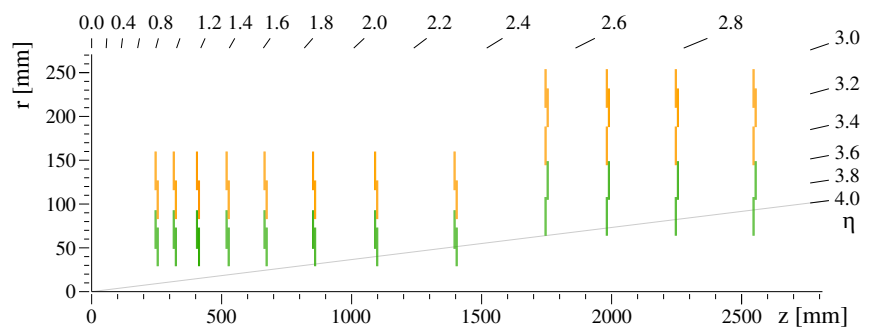
\includegraphics[width=0.6\columnwidth]{./tepx.png}
  \caption{ \onehalfspacing Sketch of the TFPX and TEPX layouts, showing one quarter of the detector in r-z view. Modules of type 1 $\times$ 2 are shown in green, while 2 $\times$ 2 modules are represented in orange. The two layers of modules that populate the front- and back-side of a disc and that overlap in $r-\phi$ can be seen by zooming into the figure in the online version. \cite{}.}
  \label{fig:CMS}
\end{figure}


\begin{figure}[H]
  \centering
  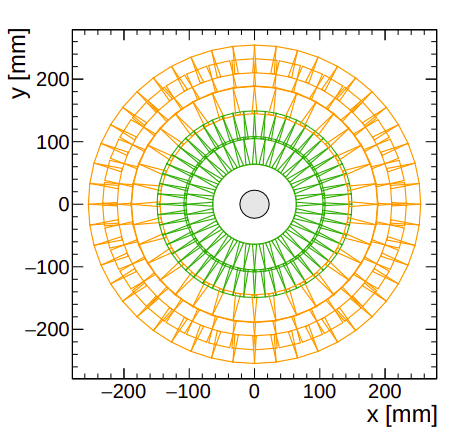
\includegraphics[width=0.5 \columnwidth]{./xydisc.png}
  \caption{ \onehalfspacing Sketch of the TEPX Disk layouts in x-y view. Modules of type 1 $\times$ 2 are shown in green, while 2 $\times$ 2 modules are represented in orange.}
  \label{fig:CMS}
\end{figure}



\begin{figure}[H]
  \centering
  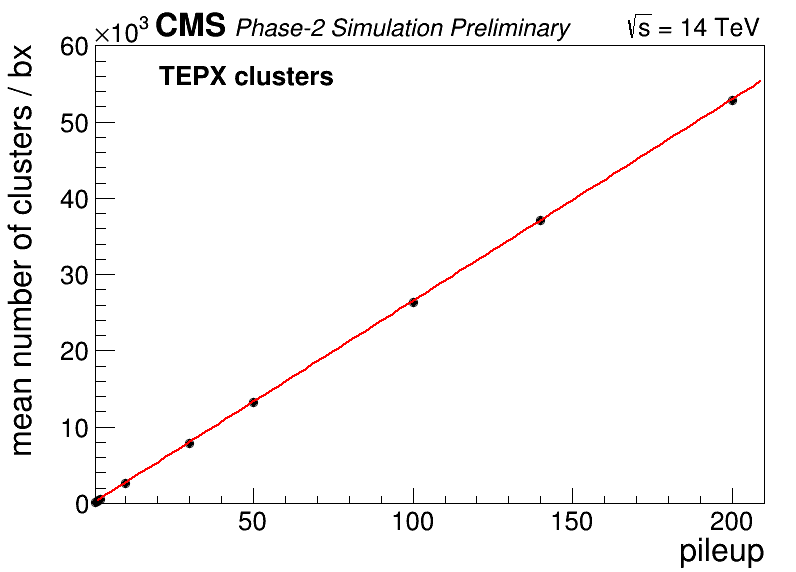
\includegraphics[width=0.5\columnwidth]{./TEPX_totalcluster_linearity.png}
  \caption{Simulated mean number of clusters for all entire TEPX detector as a function of pileup. A line is fitted between pileup values of 0 and 2, and then extrapolated up to a pileup of 200.}
  \label{fig:CMS}
\end{figure}


\begin{figure}[H]
  \centering
  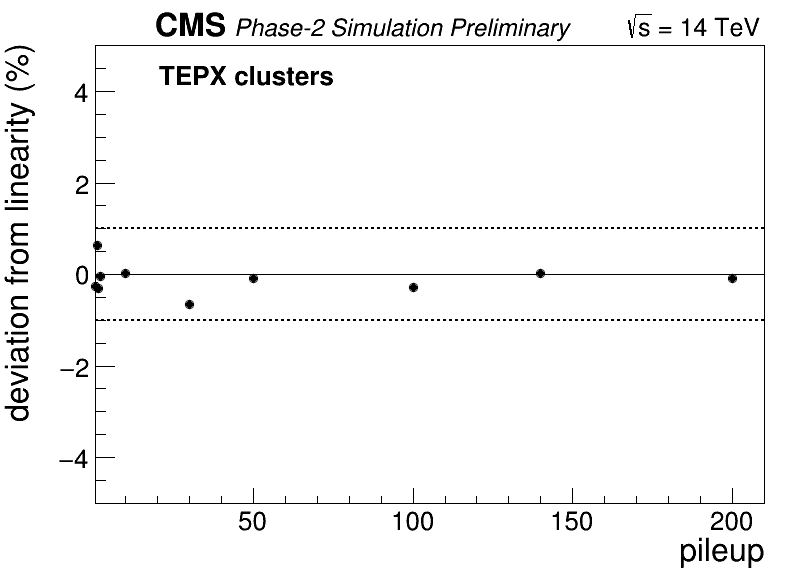
\includegraphics[width=0.5\columnwidth]{./TEPX_totalcluster_residuals.png}
  \caption{Deviation from linearity for clusters for entire TEPX detector. The non-linearity is calculated as the relative difference between the data points and the values of the fit function at the respective pileup value. Non-linearity is within 1 \% for entire pileup range. Pileup 200 corresponds to High Luminosity (HL)-LHC environment.}
  \label{fig:CMS}
\end{figure}



\begin{figure}[H]
  \centering
  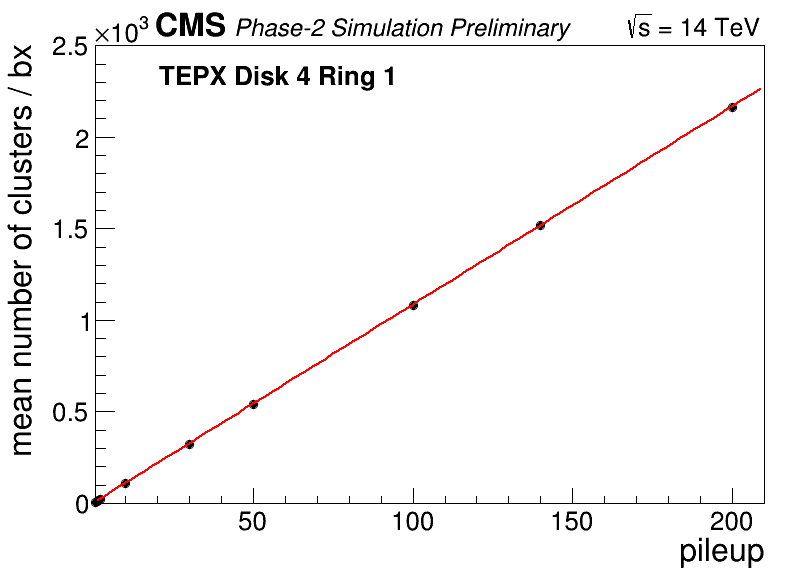
\includegraphics[width=0.5\columnwidth]{./TEPX_Disk_4_Ring_1_mean_number_of_clusters___bx_Linearity.png}
  \caption{Simulated mean number of clusters for TEPX Disk 4 Ring 1 as a function of pileup.}
  \label{fig:CMS}
\end{figure}



\begin{figure}[H]
  \centering
  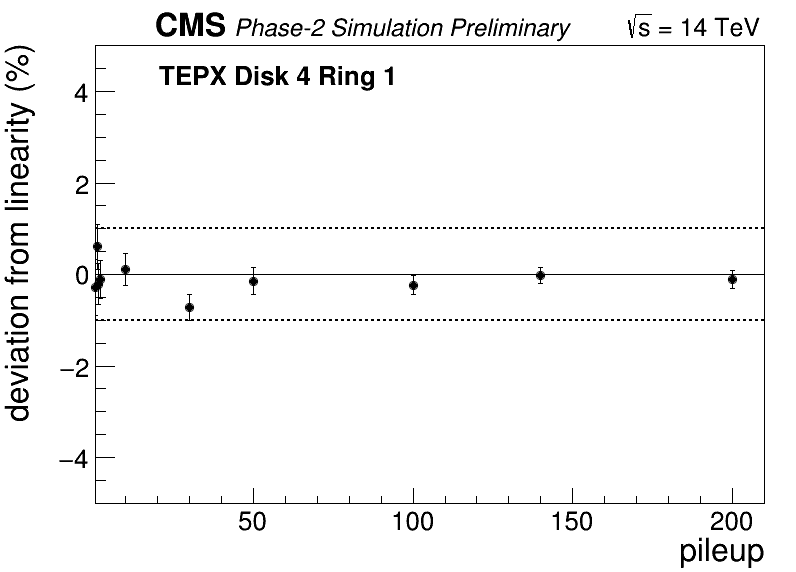
\includegraphics[width=0.5\columnwidth]{./TEPX_Disk_4_Ring_1_mean_number_of_clusters___bx_Linearity_residuals.png}
  \caption{Deviation from linearity for clusters for TEPX Disk 4 Ring 1. The non-linearity is calculated as the relative difference between the data points and the values of the fit function at the respective pileup value.}
  \label{fig:CMS}
\end{figure}






\begin{figure}[H]
  \centering
  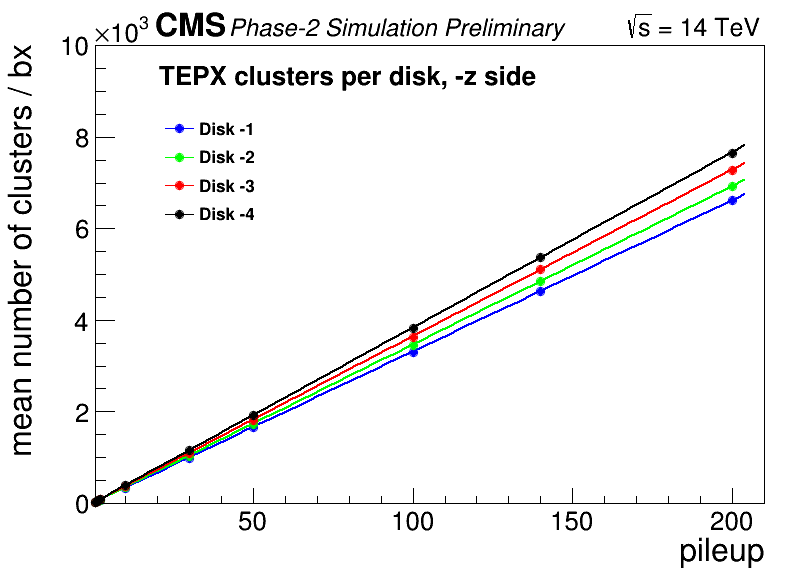
\includegraphics[width=0.5\columnwidth]{./TEPX_clusters_negativez_Linearity.png}
  \caption{Simulated mean number of clusters for -z side TEPX disks as a function of pileup.}
  \label{fig:CMS}
\end{figure}


\begin{figure}[H]
  \centering
  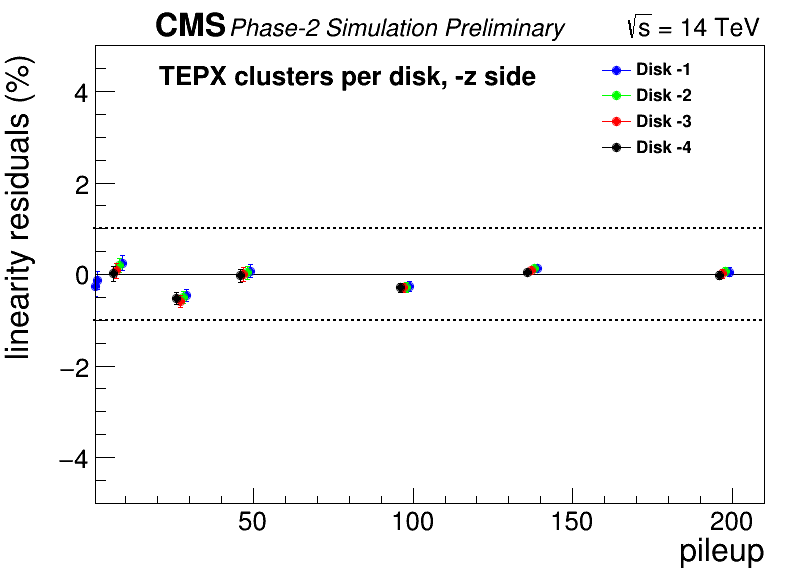
\includegraphics[width=0.5\columnwidth]{./TEPX_clusters_per_disk_negativez_Linearity_residuals.png}
  \caption{Deviation from linearity for clusters for -z side TEPX disks.}
  \label{fig:CMS}
\end{figure}

\begin{figure}[H]
  \centering
  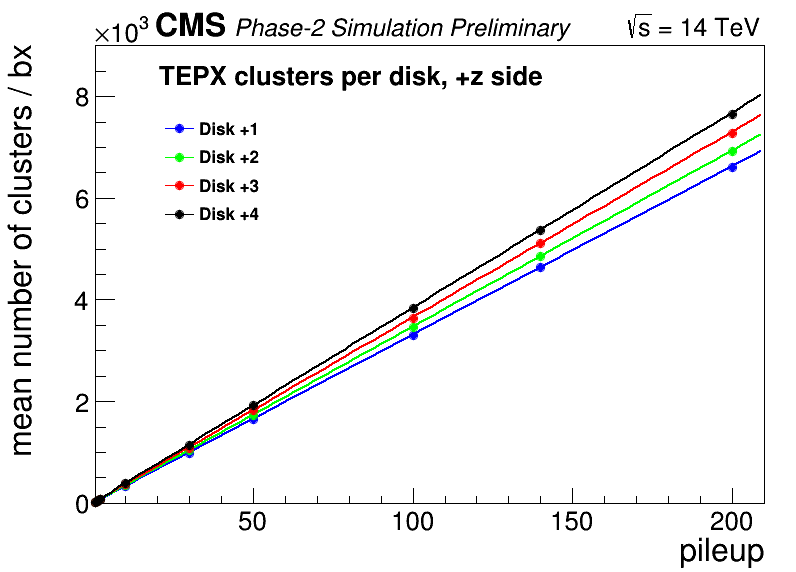
\includegraphics[width=0.5\columnwidth]{./TEPX_clusters_per_disk_positivez_linearity.png}
  \caption{Simulated mean number of clusters for +z side TEPX disks as a function of pileup.}
  \label{fig:CMS}
\end{figure}


\begin{figure}[H]
  \centering
  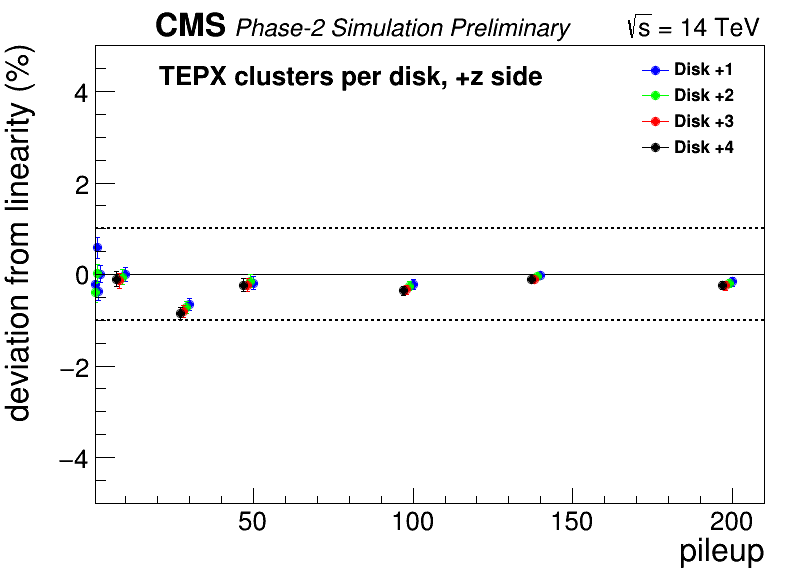
\includegraphics[width=0.5\columnwidth]{./TEPX_clusters_per_disk_postivez_Linearity_residuals.png}
  \caption{Deviation from linearity for clusters for +z side TEPX disks.}
  \label{fig:CMS}
\end{figure}

\begin{figure}[H]
  \centering
  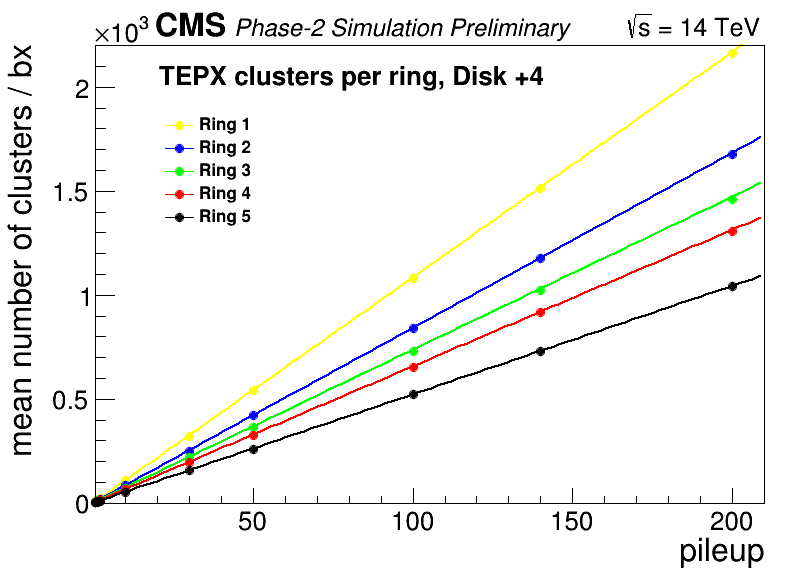
\includegraphics[width=0.5\columnwidth]{./TEPX_clusters_per_ringDisk4_Linearity.png}
  \caption{Simulated mean number of clusters for TEPX Disk 4 all rings as a function of pileup. Ring 1 has highest slope and Ring 5 has least slope.}
  \label{fig:CMS}
\end{figure}


\begin{figure}[H]
  \centering
  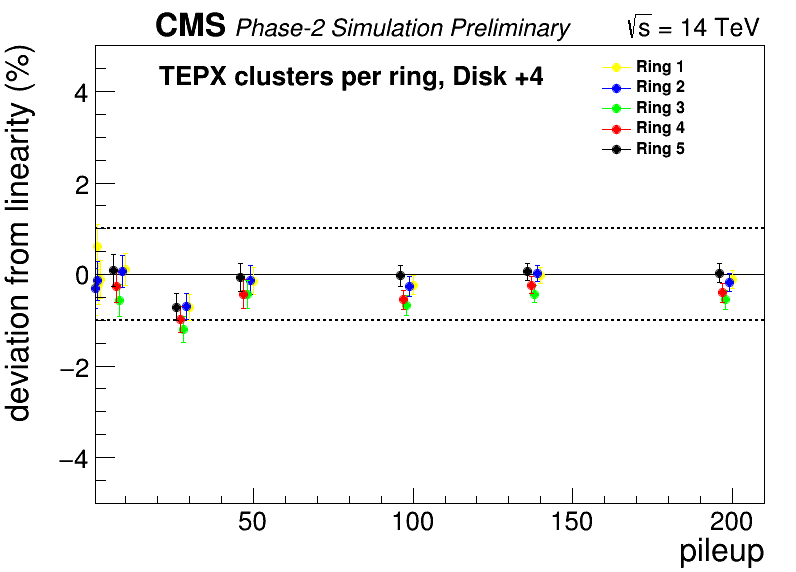
\includegraphics[width=0.5\columnwidth]{./TEPX_clusters_per_ringDisk4_Linearity_residuals.png}
  \caption{Deviation from linearity for clusters for TEPX Disk 4 all rings. Non-linearity is within $1\%$ for all rings over entire pileup range.}
  \label{fig:CMS}
\end{figure}








\begin{figure}[H]
  \centering
  \includegraphics[width=0.5\columnwidth]{./TEPX_coincidences_mean_number_of_coincidences___bx_Linearity.png}
  \caption{Simulated mean number of coincidences in $\phi$ and r for all entire TEPX detector as a function of pileup. A line is fitted between pileup values of 0 and 2, and then extrapolated up to a pileup of 200.}
  \label{fig:CMS}
\end{figure}


\begin{figure}[H]
  \centering
  \includegraphics[width=0.5\columnwidth]{./TEPX_coincidences_mean_number_of_coincidences___bx_Linearity_residuals.png}
  \caption{Deviation from linearity for coincidence in $\phi$ and r for entire TEPX detector. The non-linearity is calculated as
the relative difference between the data points and the values of the fit function at the respective pileup value.
Non-linearity is within 1 \% for entire pileup range. Pileup 200 corresponds to High Luminosity (HL)-LHC
environment.}
  \label{fig:CMS}
\end{figure}




\begin{figure}[H]
  \centering
  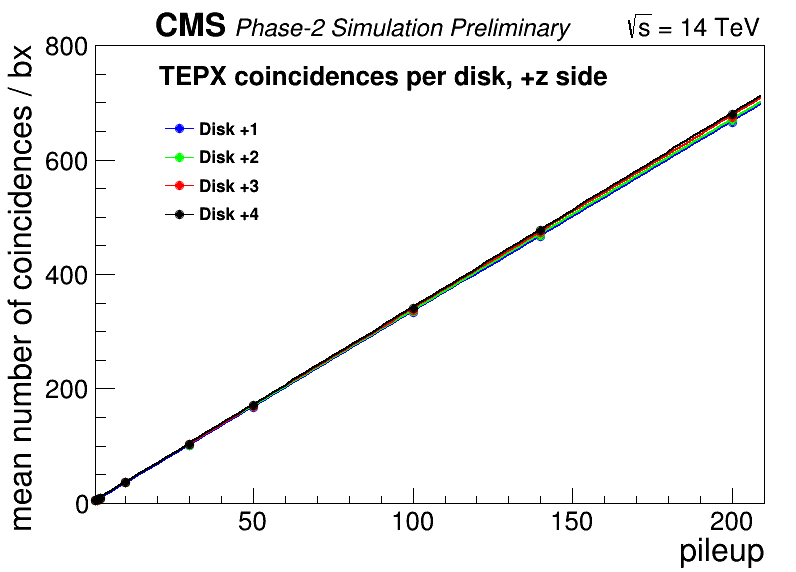
\includegraphics[width=0.5\columnwidth]{./TEPX_coincidences_per_disk__pz_side_mean_number_of_coincidences___bx_Linearity.png}
  \caption{Simulated mean number of coincidences in $\phi$ and r for +z side TEPX disks as a function of pileup.}
  \label{fig:CMS}
\end{figure}


\begin{figure}[H]
  \centering
  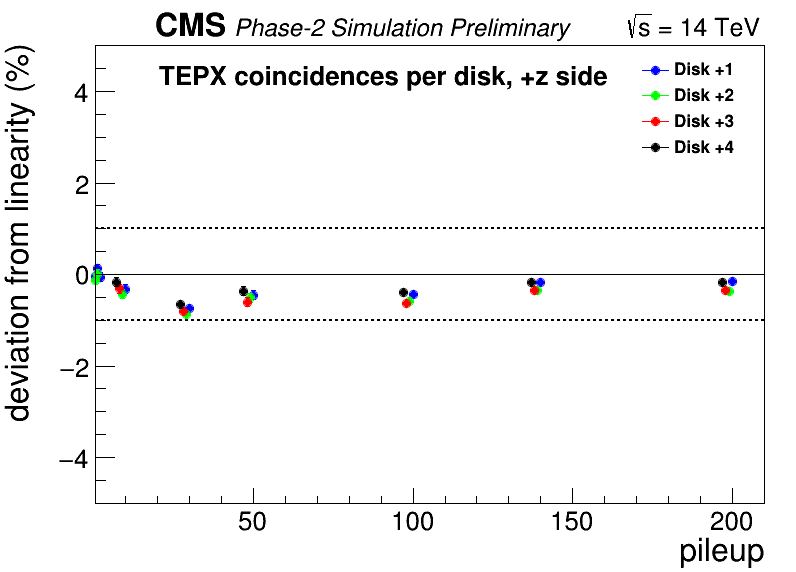
\includegraphics[width=0.5\columnwidth]{./TEPX_coincidences_per_disk__pz_side_mean_number_of_coincidences___bx_Linearity_residuals.png}
  \caption{Deviation from linearity for coincidences in $\phi$ and r for +z side TEPX disks.}
  \label{fig:CMS}
\end{figure}


\begin{figure}[H]
  \centering
  \includegraphics[width=0.5\columnwidth]{./TEPX_coincidences_per_disk,_-z_side_Linearity.png}
  \caption{Simulated mean number of coincidences in $\phi$ and r for -z side TEPX disks as a function of pileup.}
  \label{fig:CMS}
\end{figure}


\begin{figure}[H]
  \centering
  \includegraphics[width=0.5\columnwidth]{./TEPX_coincidences_per_disk,_-z_side_Linearity_residuals.png}
  \caption{Deviation from linearity for coincidences in $\phi$ and r for -z side TEPX disks.}
  \label{fig:CMS}
\end{figure}


\begin{figure}[H]
  \centering
  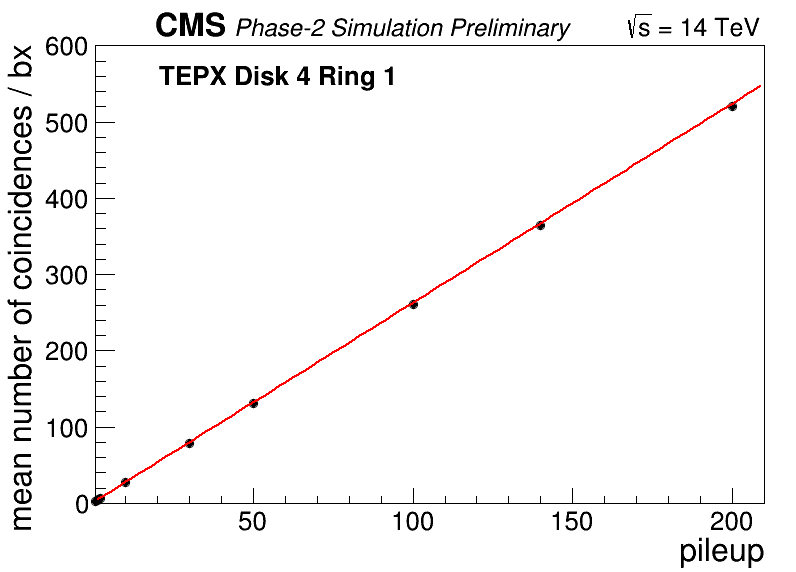
\includegraphics[width=0.5\columnwidth]{./TEPX_Disk_4_Ring_1_mean_number_of_coincidences___bx_Linearity.png}
  \caption{Simulated mean number of coincidences in $\phi$ and r for TEPX Disk 4 Ring 1 as a function of pileup.}
  \label{fig:CMS}
\end{figure}


\begin{figure}[H]
  \centering
  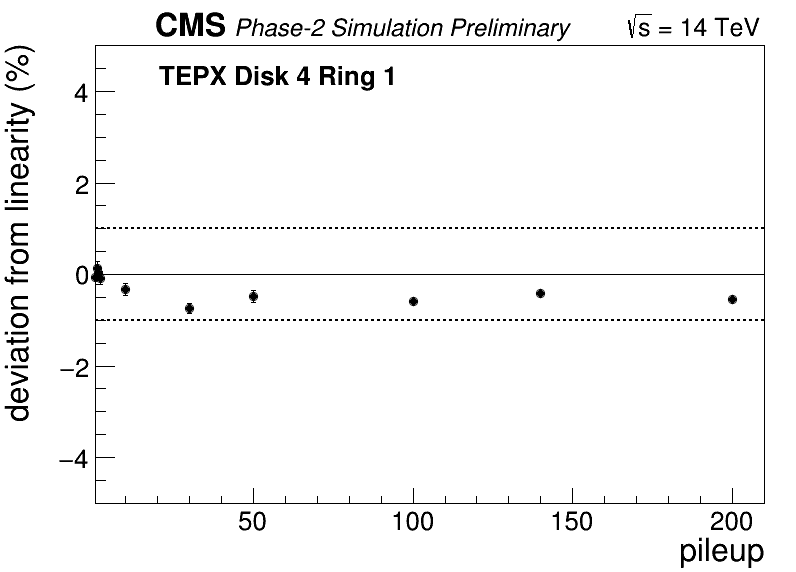
\includegraphics[width=0.5\columnwidth]{./TEPX_Disk_4_Ring_1_mean_number_of_coincidences___bx_Linearity_residuals.png}
  \caption{Deviation from linearity for coincidences in $\phi$ and r for TEPX Disk 4 Ring 1. The non-linearity is calculated as the
relative difference between the data points and the values of the fit function at the respective pileup value.}
  \label{fig:CMS}
\end{figure}


\begin{figure}[H]
  \centering
  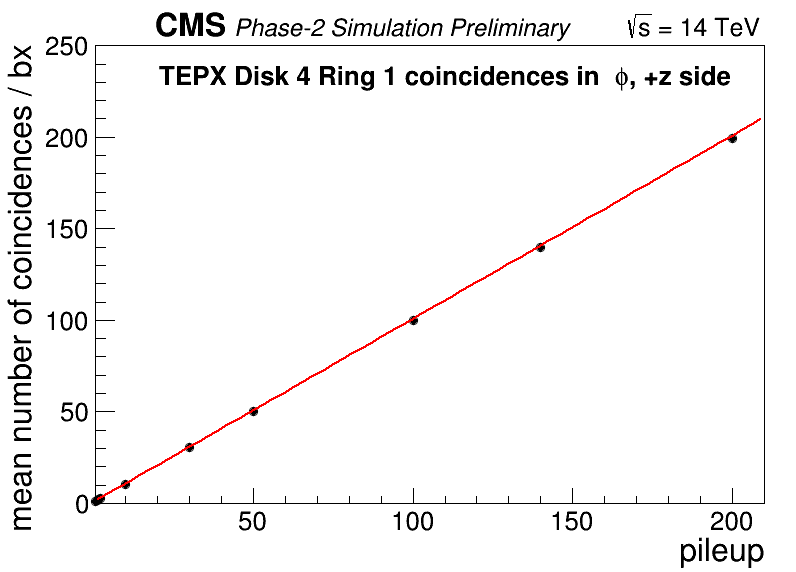
\includegraphics[width=0.5\columnwidth]{./TEPX_Disk_4_Ring_1_coincidences_in_phi__pz_side_mean_number_of_coincidences___bx_Linearity.png}
  \caption{Simulated mean number of coincidences in $\phi$ for TEPX +z side Disk 4 Ring 1 as a function of pileup.}
  \label{fig:CMS}
\end{figure}


\begin{figure}[H]
  \centering
  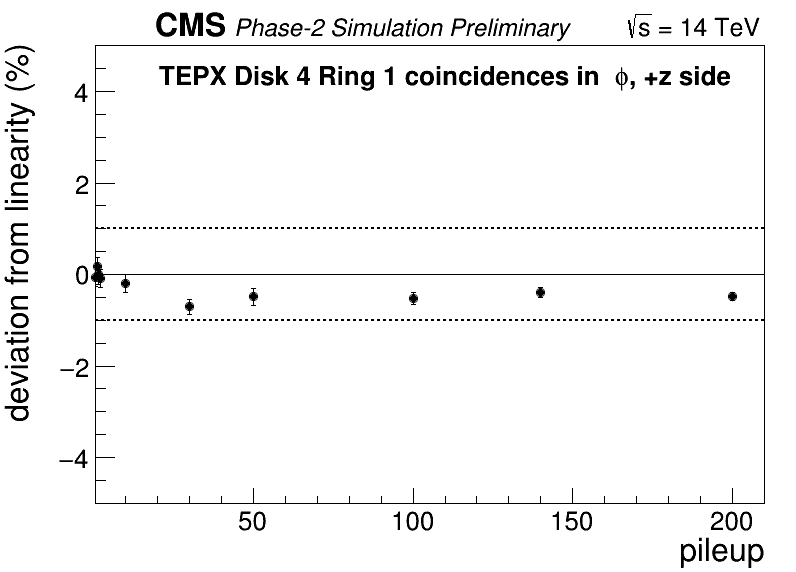
\includegraphics[width=0.5\columnwidth]{./TEPX_Disk_4_Ring_1_coincidences_in_phi__pz_side_mean_number_of_coincidences___bx_Linearity_residuals.png}
  \caption{Deviation from linearity for coincidences in $\phi$ for TEPX +z side Disk 4 Ring 1. The non-linearity is calculated as the relative difference between the data points and the values of the fit function at the respective pileup value.}
  \label{fig:CMS}
\end{figure}



\begin{figure}[H]
  \centering
  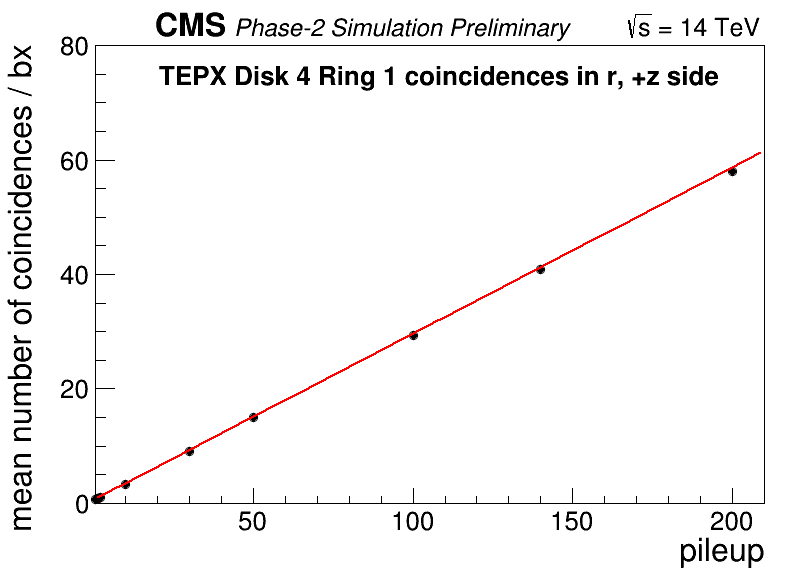
\includegraphics[width=0.5\columnwidth]{./TEPX_Disk_4_Ring_1_coincidences_in_r__pz_side_mean_number_of_coincidences___bx_Linearity.png}
  \caption{Simulated mean number of coincidences in r for TEPX +z side Disk 4 Ring 1 as a function of pileup.}
  \label{fig:CMS}
\end{figure}


\begin{figure}[H]
  \centering
  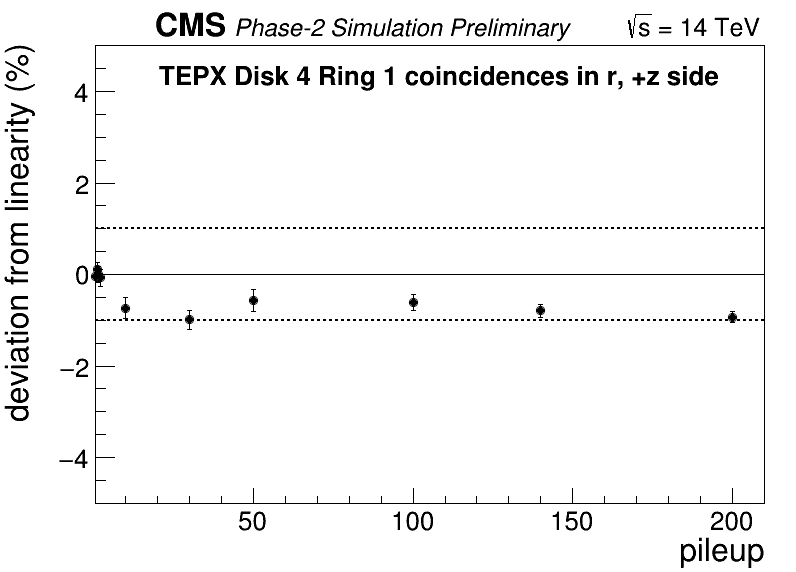
\includegraphics[width=0.5\columnwidth]{./TEPX_Disk_4_Ring_1_coincidences_in_r__pz_side_mean_number_of_coincidences___bx_Linearity_residuals.png}
  \caption{Deviation from linearity for coincidences in r for TEPX +z side Disk 4 Ring 1. The non-linearity is calculated as the relative difference between the data points and the values of the fit function at the respective pileup value.}
  \label{fig:CMS}
\end{figure}



\begin{figure}[H]
  \centering
  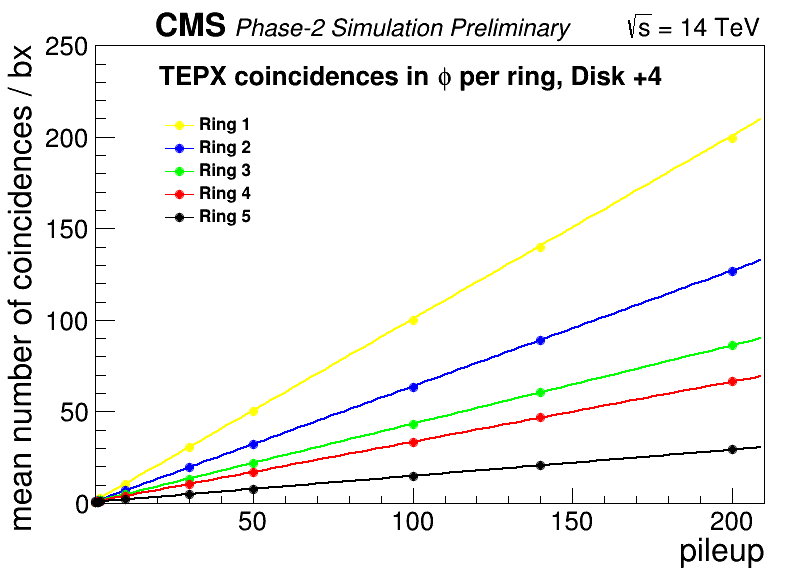
\includegraphics[width=0.5\columnwidth]{./TEPX_coincidences_in_phi_per_ring_mean_number_of_coincidences___bxDisk4_Linearity.png}
  \caption{Simulated mean number of coincidences in $\phi$ for +z side TEPX Disk 4 per ring as a function of pileup. Ring 1 has highest slope and Ring 5 has least slope.}
  \label{fig:CMS}
\end{figure}



\begin{figure}[H]
  \centering
  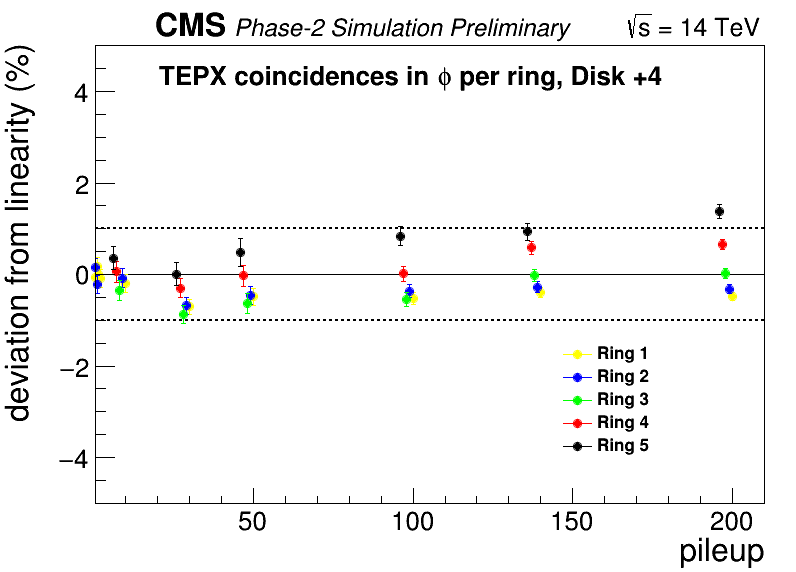
\includegraphics[width=0.5\columnwidth]{./TEPX_coincidences_in_phi_per_ring_mean_number_of_coincidences___bxDisk4_Linearity_residuals.png}
  \caption{Deviation from linearity for coincidences in $\phi$ for +z side TEPX Disk 4 per ring. Non-linearity is within 1\% for all rings over entire pileup range.}
  \label{fig:CMS}
\end{figure}



\begin{figure}[H]
  \centering
  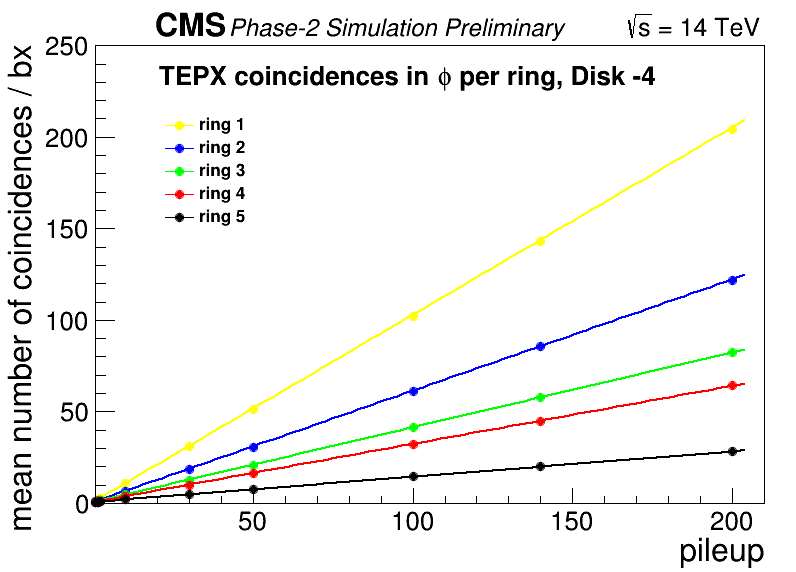
\includegraphics[width=0.5\columnwidth]{./TEPX_coincidences_inphi_per_ring__Disk_-4_Linearity.png}
  \caption{Simulated mean number of coincidences in \phi for -z side TEPX Disk 4 per ring as a function of pileup. Ring 1 has highest slope and Ring 5 has least slope.}
  \label{fig:CMS}
\end{figure}


\begin{figure}[H]
  \centering
  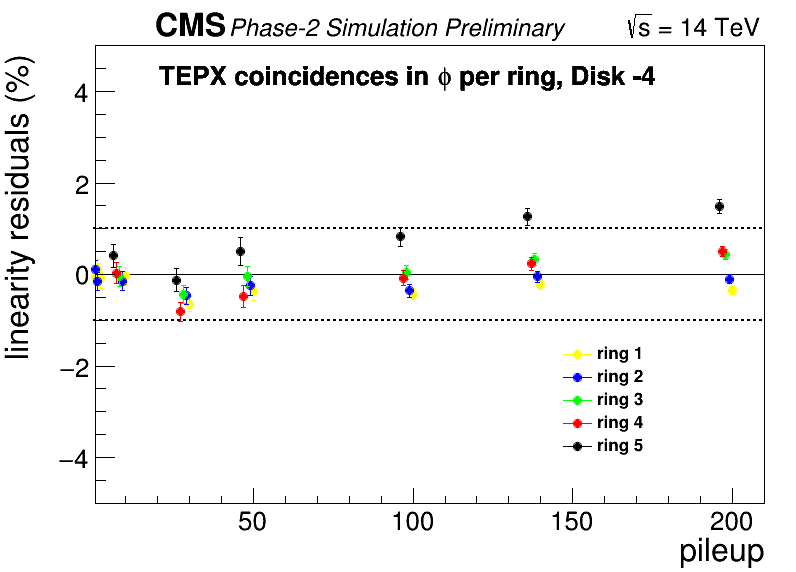
\includegraphics[width=0.5\columnwidth]{./TEPX_coincidences_inphi_per_ring__Disk_-4_Linearity_residuals.png}
  \caption{Deviation from linearity for coincidences in $\phi$ for -z side TEPX Disk 4 per ring. Non-linearity is within 1\% for all rings over entire pileup range.}
  \label{fig:CMS}
\end{figure}



\begin{figure}[H]
  \centering
  \includegraphics[width=0.5\columnwidth]{./TEPX_coincidences_in_r_per_ring__Disk_-4_Linearity.png}
  \caption{Simulated mean number of coincidences in r for -z side TEPX Disk 4 per ring as a function of pileup. Ring 1 has highest slope and Ring 5 has least slope.}
  \label{fig:CMS}
\end{figure}


\begin{figure}[H]
  \centering
  \includegraphics[width=0.5\columnwidth]{./TEPX_coincidences_in_r_per_ring__Disk_-4_Linearity_residuals.png}
  \caption{Deviation from linearity for coincidences in $\phi$ for -z side TEPX Disk 4 per ring. Non-linearity is within 1\% for all rings over entire pileup range.}
  \label{fig:CMS}
\end{figure}


\begin{figure}[H]
  \centering
  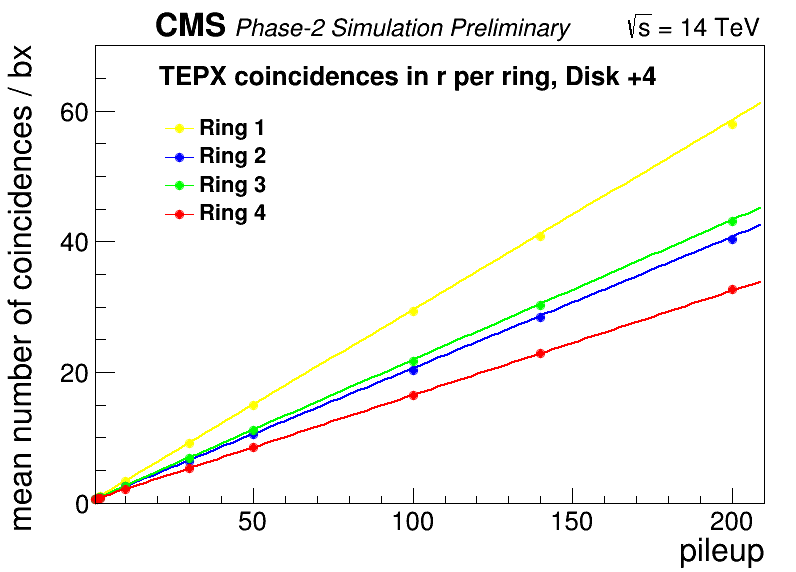
\includegraphics[width=0.5\columnwidth]{./TEPX_coincidences_in_r_per_ring_mean_number_of_coincidences___bxDisk4_Linearity.png}
  \caption{Simulated mean number of coincidences in r for +z side TEPX Disk 4 per ring as a function of pileup. Ring 1 has highest slope and Ring 5 has least slope.}
  \label{fig:CMS}
\end{figure}


\begin{figure}[H]
  \centering
  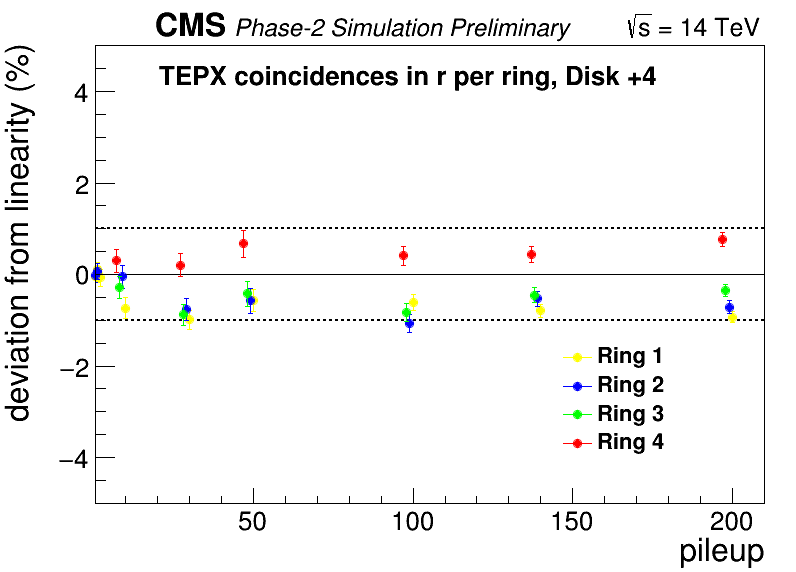
\includegraphics[width=0.5\columnwidth]{./TEPX_coincidences_in_r_per_ring_mean_number_of_coincidences___bxDisk4_Linearity_residuals.png}
  \caption{Deviation from linearity for coincidences in r for +z side TEPX Disk 4 per ring. Non-linearity is within 1\% for all rings over entire pileup range.}
  \label{fig:CMS}
\end{figure}
